\documentclass{article}
\usepackage[utf8]{inputenc}
\usepackage[english]{babel}
\usepackage[font=small,labelfont=bf]{caption}
\usepackage{geometry}
\usepackage{natbib}
\usepackage{pxfonts}
\usepackage{graphicx}
\usepackage{newfloat}
\usepackage{setspace}
\usepackage{placeins}
%\doublespacing

\newcommand{\argmax}{\mathop{\mathrm{argmax}}\limits}

\title{\textit{Supporting Information for}: Memory for television episodes preserves event content while introducing new across-event similarities}
\author{Andrew C. Heusser\textsuperscript{1, 2}, Paxton C. Fitzpatrick\textsuperscript{1}, and Jeremy R. Manning\textsuperscript{1, *}\\\textsuperscript{1}Department of Psychological and Brain Sciences\\Dartmouth College, Hanover, NH 03755, USA\\\textsuperscript{2}Akili Interactive\\Boston, MA 02110\\\textsuperscript{*}Corresponding author: jeremy.r.manning@dartmouth.edu}

\bibliographystyle{apa}

\begin{document}
\maketitle

\setcounter{equation}{0}
\setcounter{figure}{0}
\setcounter{table}{0}
\setcounter{page}{1}
\setcounter{section}{0}
\makeatletter
\renewcommand{\theequation}{S\arabic{equation}}
\renewcommand{\thefigure}{S\arabic{figure}}
\renewcommand{\bibnumfmt}[1]{[S#1]}
\renewcommand{\citenumfont}[1]{S#1}


\section*{Overview}
This document provides additional details about the methods we used in the main text.  We also include some additional analyses referenced in the main text.

\section*{Additional details about topic modeling methods and results}
\subsection*{Optimizing topic model parameters}
In order to create accurate video and recall models, we used an optimization method that was driven by our ability to explain hand-annotated memory performance metrics collected by \cite{ChenEtal17}.  Specifically, we used a grid search to compute the $\omega$ (video sliding window duration, in scenes), $\rho$ (recall sliding window duration, in sentences), and $K$ (number of topics) that satisfied
\[
\argmax_{\omega, \rho, K} \left[\mathrm{corr}\left(\mathrm{corr}\left(\mu\left(\omega, \rho, K\right), \nu\left(\omega, \rho, K\right)\right), \theta\right)\right],
\]
where $\mathrm{corr}(\mu, \nu)$ is the per-participant correlation between the upper triangles of the temporal correlation matrices of the video ($\mu$) and recall ($\nu$) trajectory, and $\theta$ is the per-participant hand-annotated memory performance.  We searched over a grid of pre-specified values for each of these parameters; the resulting correlations are displayed in Figure~\ref{fig:paramsearch}.  The optimal parameters were $\omega = 50$, $\rho = 10$, and $K = 100$.


\begin{figure}[p!]
\centering
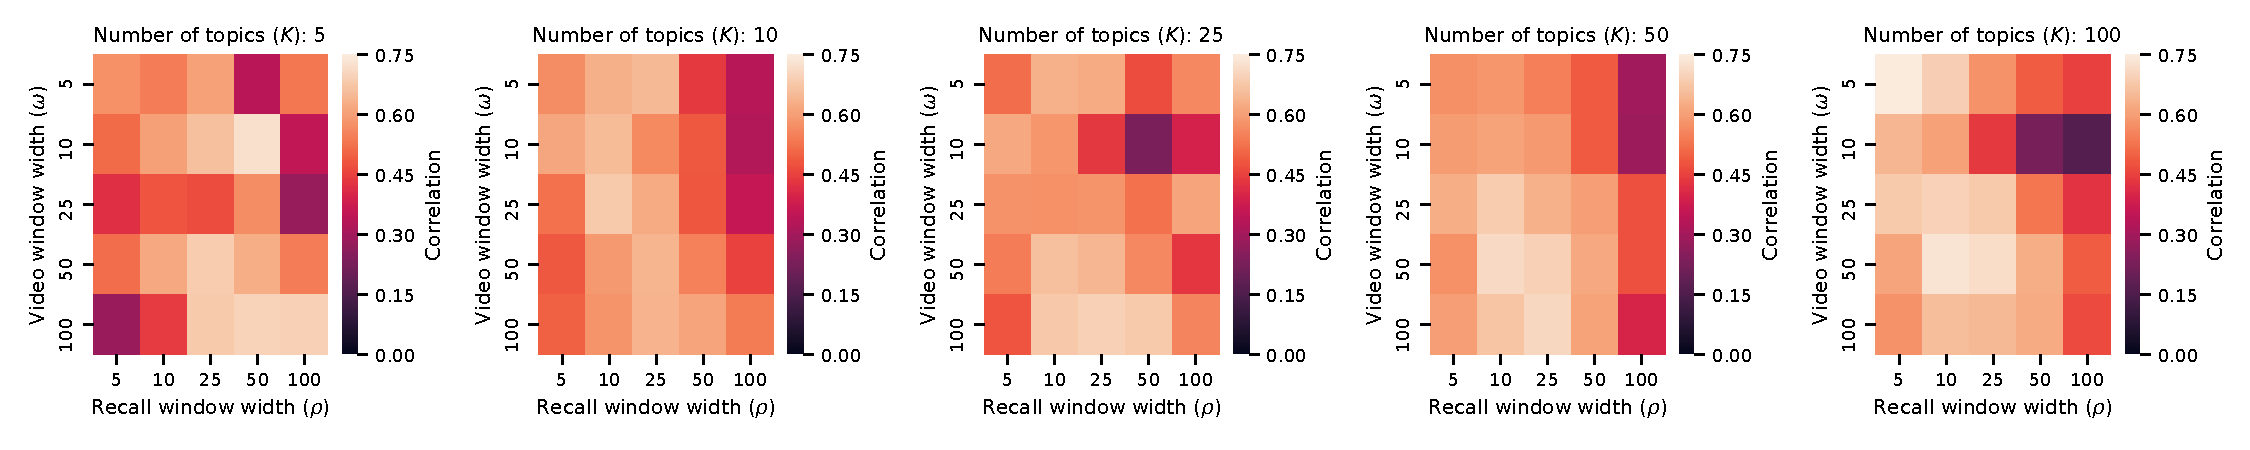
\includegraphics[width=1\textwidth]{figs/parameter_search}
\caption{\small \textbf{Optimizing topic model parameters.}  We performed a grid search over video sliding window length ($\omega \in \{5, 10, 25, 50, 100 \}$), recall sliding window length ($\rho \in \{5, 10, 25, 50, 100 \}$, and number of topics ($K \in \{5, 10, 25, 50, 100 \}$.  The reported correlations are between per-subject video-recall trajectory correlations and per-subject hand-annotated memory performance ratings.}
\label{fig:paramsearch}
\end{figure}

The optimized model converged on 32 unique topics that were assigned non-zero weights over the course of the video.  We provide a list of the top ten highest-weighted words from each topic in Figure~\ref{fig:topics}.

\begin{figure}[p!]
\centering
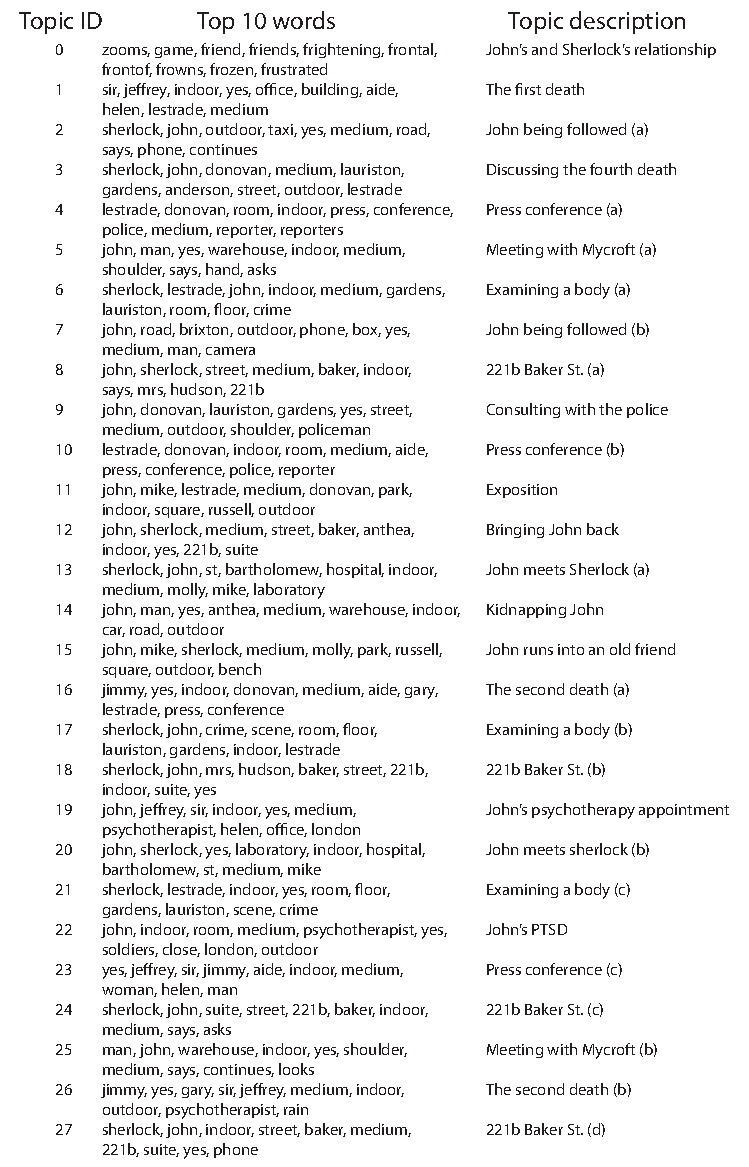
\includegraphics[width=0.65\textwidth]{figs/topic_words}
\caption{\small \textbf{Topics discovered in \textit{Sherlock}.} We applied a topic model to hand-annotated information about 1000 scenes spanning the 45 minute episode.  We identified 27 unique topics with non-zero weights (we used $K=100$ topics to fit the model).  Each topic comprises a distribution of weights over all words in the vocabulary.  For each topic, we show the words with the 10 largest weights, along with a suggested description of the topic.}
\label{fig:topics}
\end{figure}
\FloatBarrier

\subsection*{Feature importance analyses}
To determine the contribution of each feature to the structure of the video topic proportions, we conducted a ``leave one out'' analysis.  Specifically, we compared the original video topic trajectory (created using all hand-annotated features from the 1000 hand-annotated scenes spanning the \textit{Sherlock} episode; see \textit{Methods} for a full list of features) with video trajectories created using all but one type of feature.  We created temporal correlation matrices for each trajectory (using the topic proportions matrices) and correlated the upper triangles of each impoverished trajectory with the original feature-complete trajectory.  Observing a lower correlation between an impoverished trajectory (holding out a particular feature) and the feature-complete trajectory would suggest that the given feature played a more prominent role in shaping the temporal structure of the feature-complete trajectory.  We found that hand-annotated scene locations provided the most structure to the feature-complete trajectory, whereas the name of the character(s) in focus for each shot provided the least structure (Fig.~\ref{fig:feature-importance}A).

\begin{figure}[t]
\centering
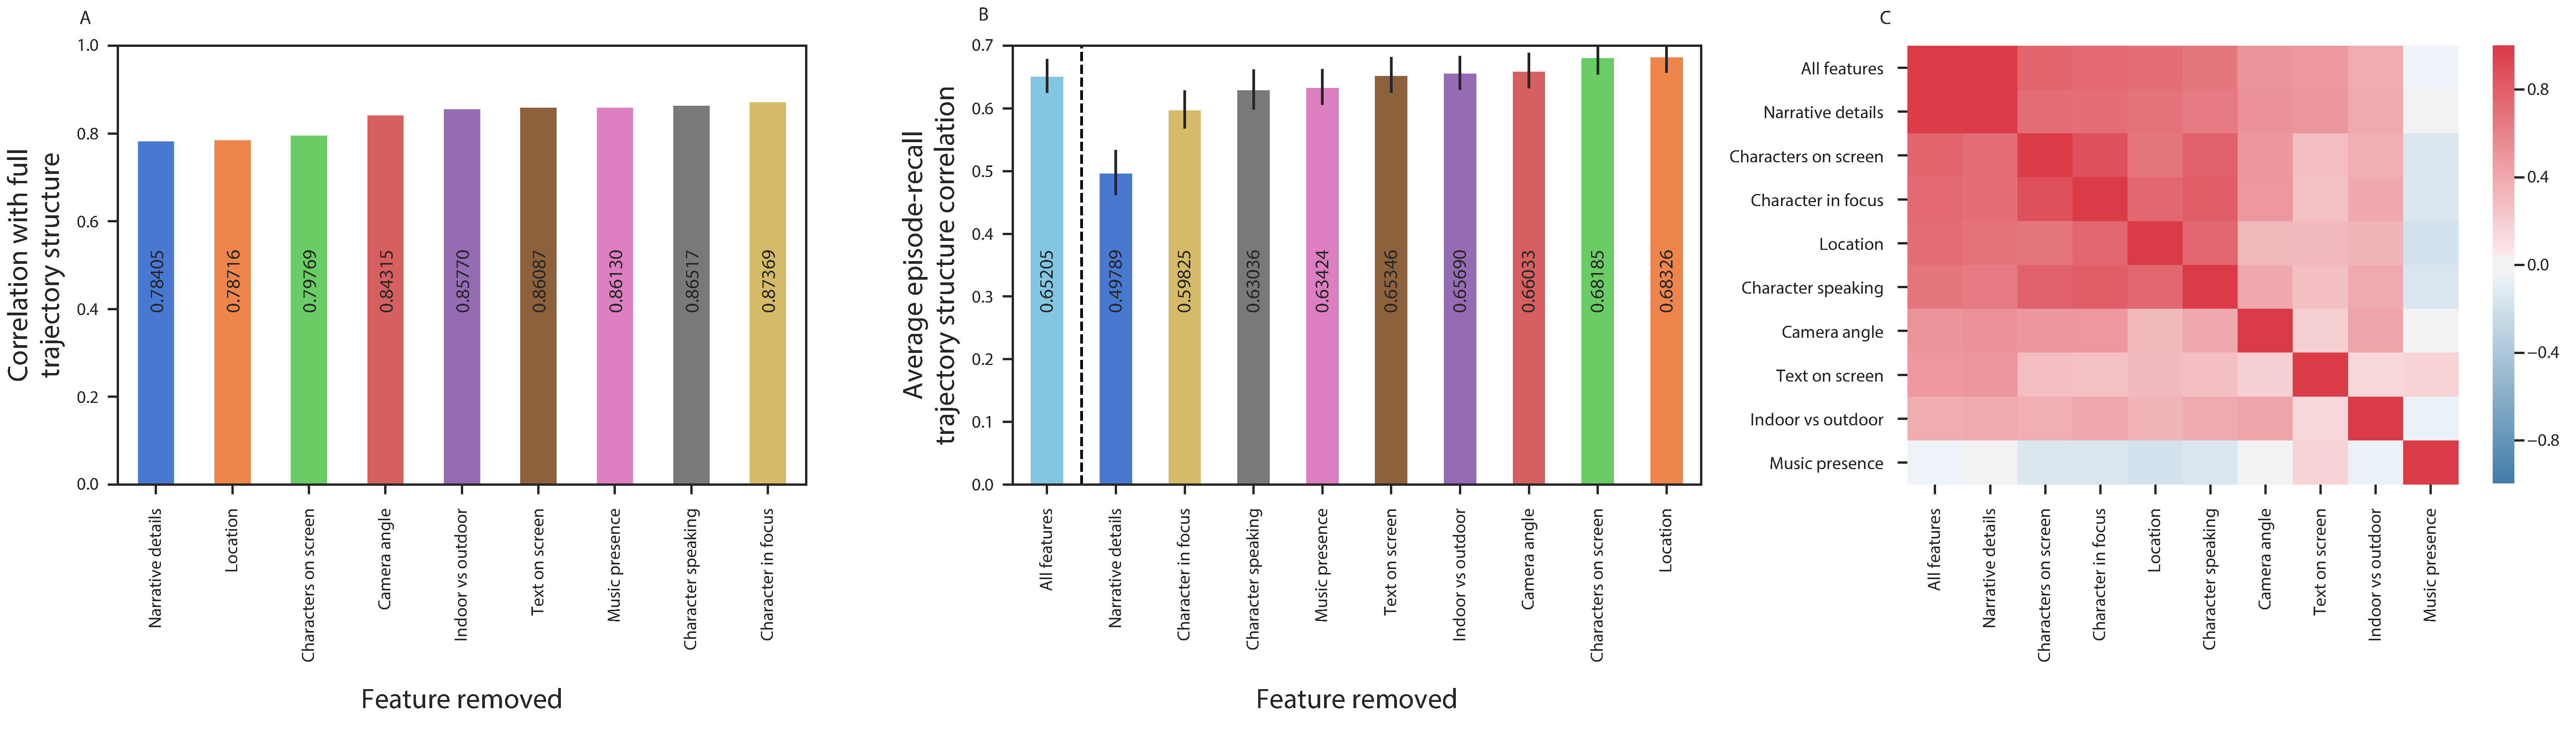
\includegraphics[width=1\textwidth]{figs/feature_value}
\caption{\small \textbf{Feature importance analysis.} \textbf{A.} Contributions of each feature type to the structure of the video trajectory. The bar heights reflect the correlation between the video trajectory computed using all features with a video trajectory computed using all features except the indicated feature.  (Lower bars reflect features that contribute more substantially to the video trajectory's shape.) \textbf{B.} Which features are preserved during recall?  The bar heights reflect the (average) across-participant correlations between the video and recall trajectories.  Error bars denote bootstrap-estimated standard error of the mean.  \textbf{C.} Feature correlation matrix.  Each entry displays the correlation between video topic trajectories created using only the indicated (row/column) features.}
\label{fig:feature-importance}
\end{figure}

We also carried out an analysis of which annotated features tended to shape aspects of the video topic trajectory's structure that were preserved in participants' recalls.  Specifically, we computed the timepoint-by-timepoint correlation matrix of the video topic trajectory, and correlated its upper triangle with that of the timepoint-by-timepoint correlation matrices of each participant's recall topic trajectory (resampled using linear interpolation to have the same number of timepoints as the video trajectory).  This yielded a single correlation coefficient for each participant.  We then repeated this analysis with each annotated feature held out in turn.  Observing a lower correlation between the video and recall trajectories (when a given feature was held out) would indicate that participants utilize changes in that feature's content to discriminate between sections of the video when organizing their recalls.  We found that hand-annotated narrative details were the most heavily utilized type of feature, whereas changes in which character was speaking tended not to impact participants' recall structures (Fig.~\ref{fig:feature-importance}B).

Next, we wondered how the different types of features might relate.  For example, knowing which character is in focus during a given scene may also provide information about which character is speaking.  We computed video topic trajectories for each feature in turn, and then compared the upper triangles of the temporal correlation matrices of all pairs of features.  This provided additional confirmation that the shape of the full trajectory (including all types of features) was largely driven by narrative details.  We also found that character-driven features (characters on screen, characters speaking, and characters in focus) were strongly correlated.  Other details, such as the presence or absence of music, led to very different topic trajectories (Fig.~\ref{fig:feature-importance}C).
\FloatBarrier

\subsection*{Creating a low-dimensional embedding space}
Figures~5 and 6C in the main text display two-dimensional projections of the 100-dimensional topic trajectories for the video (5A, 6C), average recall (5B), and each individual's recall (5C, 6C).  We created these embeddings using the Uniform Manifold Approximation and Projection algorithm \citep[UMAP;][]{McInEtal18} called from our high-dimensional visualization and text analysis software, \texttt{HyperTools}~\citep{HeusEtal18a}.  An advantage of the UMAP algorithm over comparable manifold learning techniques (such as $t$-SNE) is that UMAP explicitly attempts to preserve the global structure of the data \citep{McInEtal18,BechEtal19} by constructing a space where distance on the manifold is standard Euclidean distance, with respect to the global coordinate system.  This was important in our use case, as we wanted to visualize both the evolving structure of the video and the spatial relationships between presented and recalled content.  

UMAP achieves a balance between representing local and global structure via a subset of its hyper-parameters: \texttt{n\_neighbors} , \texttt{spread}, and \texttt{min\_dist}.  The \texttt{n\_neighbors} hyper-parameter ($K$) denotes the number of nearest neighbors to consider in constructing the high-dimensional fuzzy simplicial set for each datapoint.  \texttt{Spread} ($\gamma$) and \texttt{min\_dist} ($\delta$) function together to create the differentiable decay curve used to approximate the injective function used to map between high- and low-dimensional fuzzy simplicial sets.  In essence, \texttt{min\_dist} determines the degree to which nearby points are clustered or expanded, relative to to the overall \texttt{spread}.

To optimize the manifold space shown in Figures~5 and 6C, we performed a grid search over pre-specified values of these hyper-parameters, as well as a pre-specified set of random states ($\tau$).  Additionally, as described in \textit{Methods}, we ensured the video and recall events were projected onto the \textit{same} low-dimensional manifold by fitting the embedding model to a stacked matrix of 



\section*{Participant-level figures referenced in the main text}

\begin{figure}[p!]
\centering
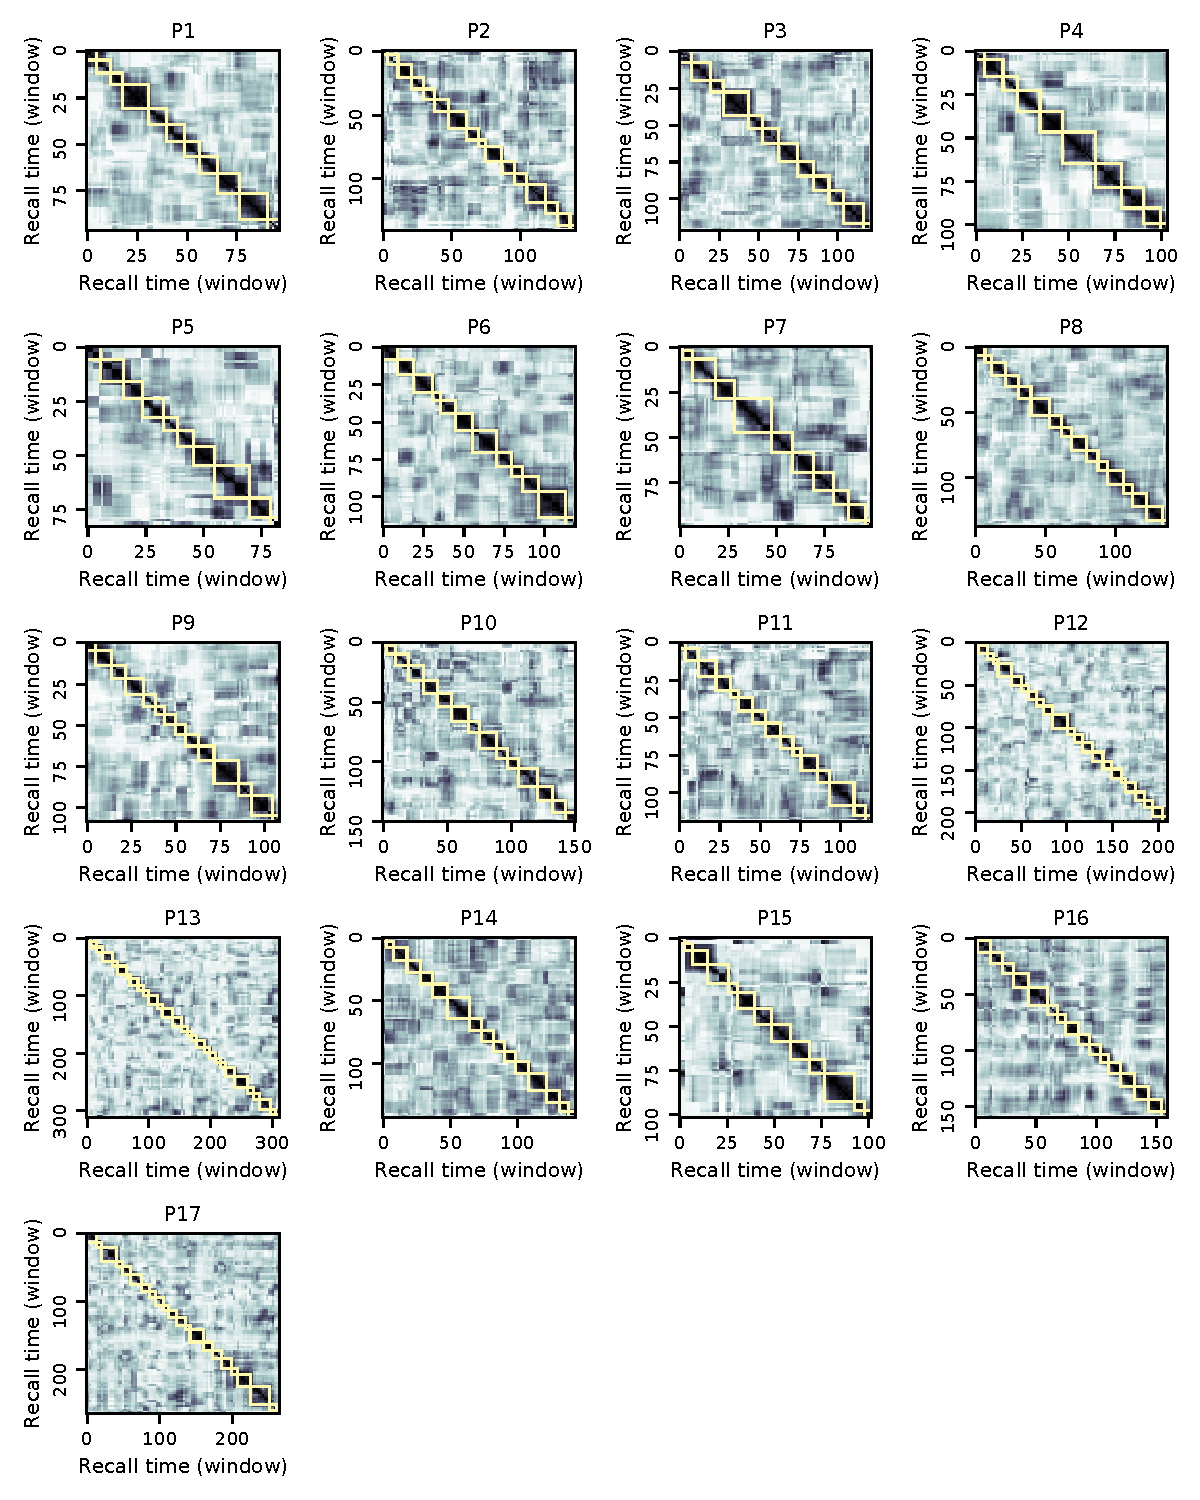
\includegraphics[width=\textwidth]{figs/corrmats}
\caption{\small \textbf{Recall trajectory temporal correlation matrices and event segmentation fits.} Each panel is in the same format as Figure~2E in the main text.  The yellow boxes indicate HMM-identified event boundaries.}
\label{fig:corrmats}
\end{figure}

\begin{figure}[p!]
\centering
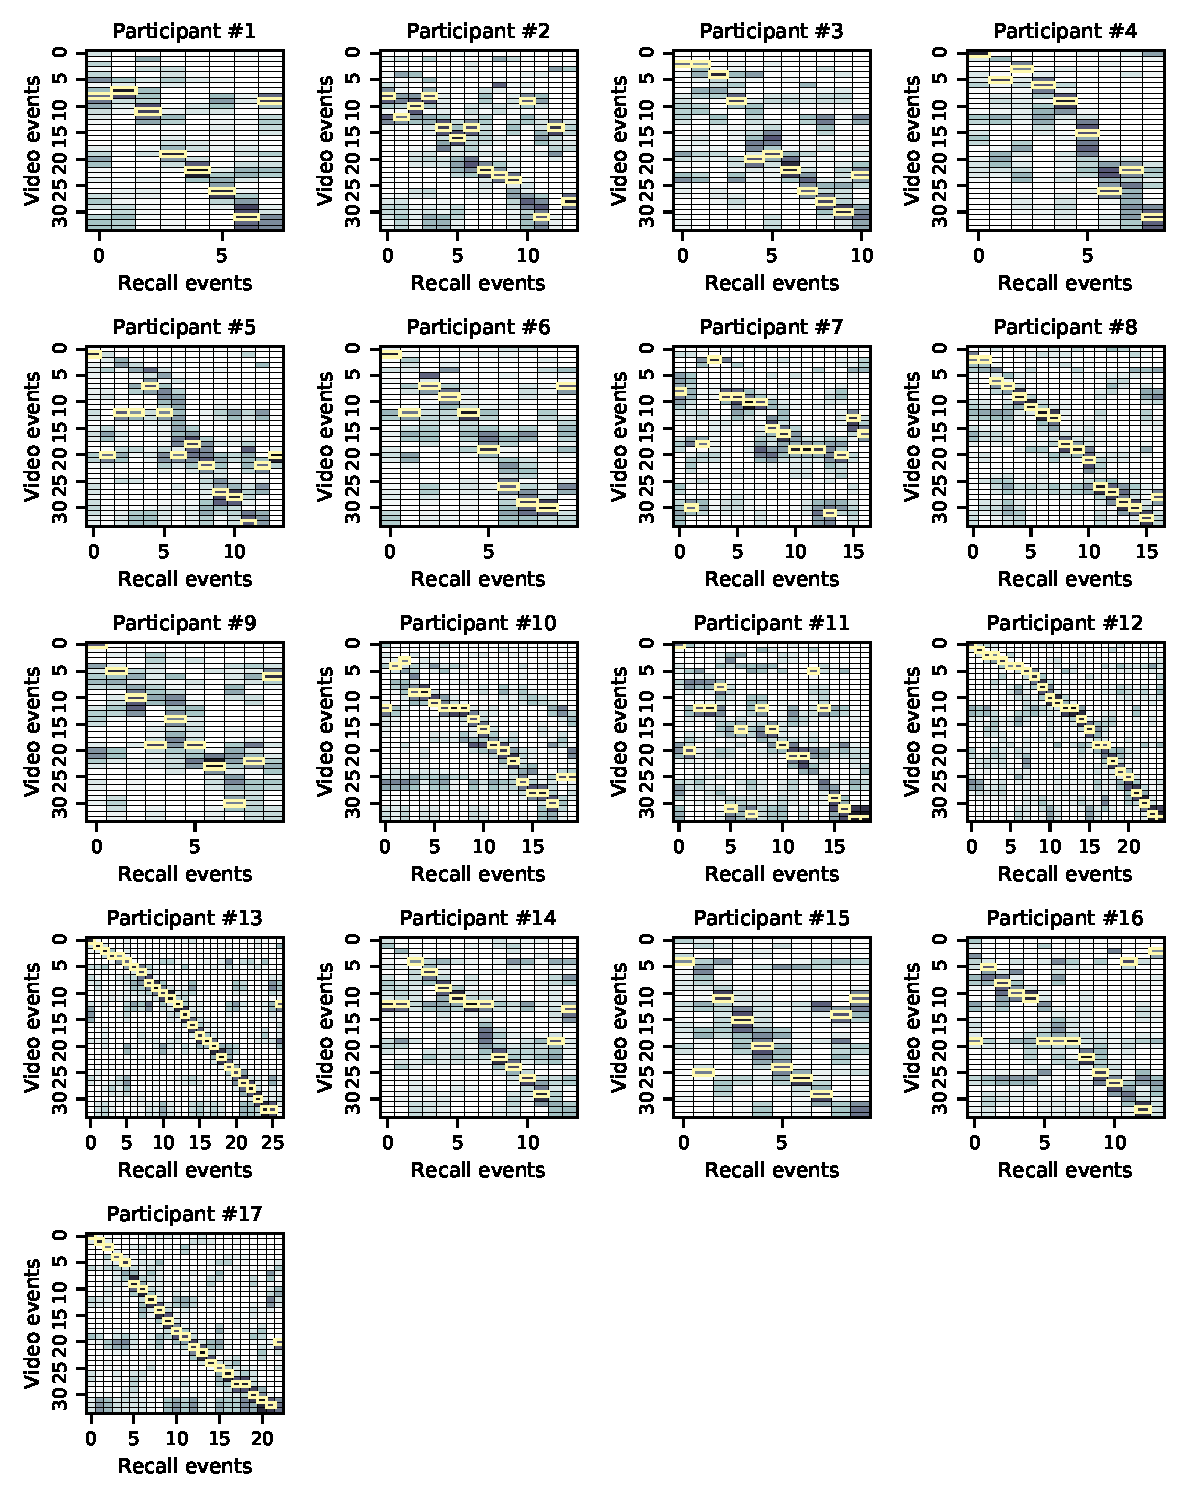
\includegraphics[width=\textwidth]{figs/matchmats}
\caption{\small \textbf{Video-recall event correlation matrices.}  Each panel is in the same format as Figure~2G in the main text.  The yellow boxes mark the maximum correlation in each column.}
\label{fig:matchmats}
\end{figure}

\begin{figure}[p!]
\centering
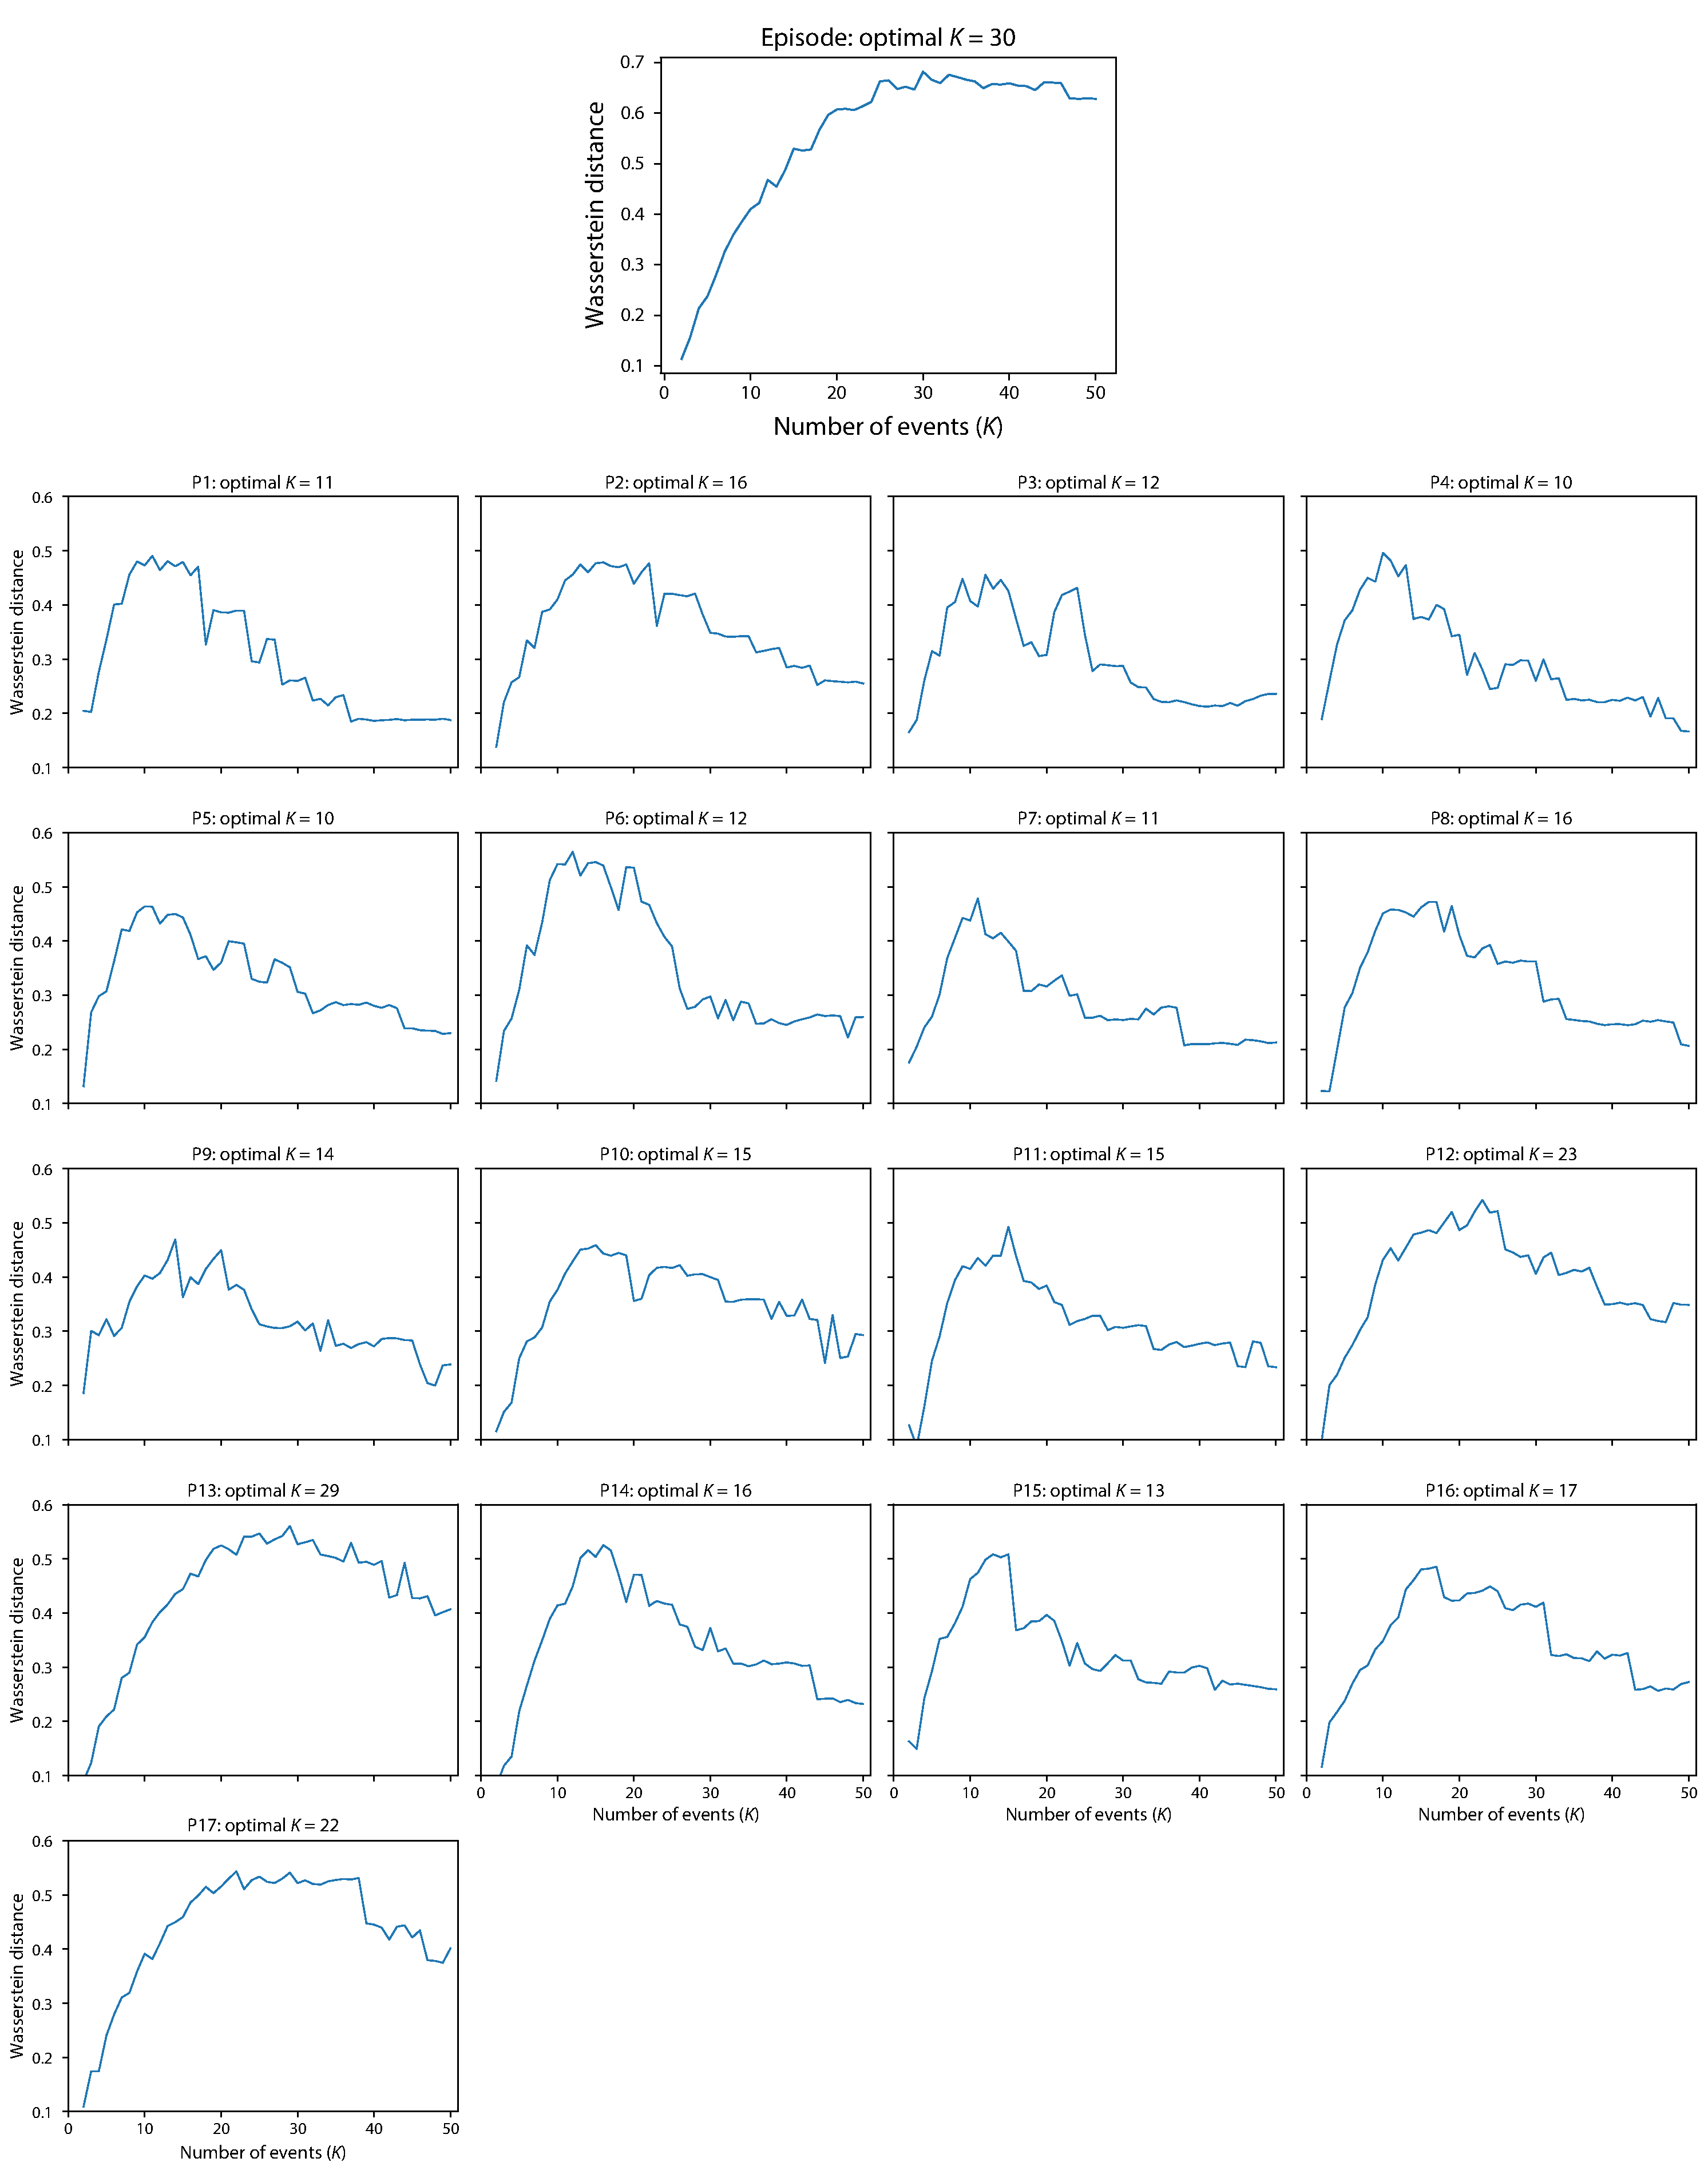
\includegraphics[width=.9\textwidth]{figs/k_optimization}
\caption{\small \textbf{Video and recall trajectory \textit{K}-optimization functions.}  We selected the optimal $K$-value for the video and each recall trajectory, using the formula described in \textit{Methods}. This computation resulted in a curve for each trajectory, describing the Wasserstein distance between the distributions of within-event and across-event topic vector correlations, as a function of $K$.}
\label{fig:k_optimization}
\end{figure}

\

\newpage
\renewcommand{\refname}{Supplemental references}
\bibliography{../../CDL-bibliography/memlab}


\end{document}
